\documentclass[11pt,letterpaper]{article}
\usepackage[utf8]{inputenc}
\usepackage[T1]{fontenc}
\usepackage[spanish,es-tabla,es-nodecimaldot]{babel}
\usepackage{lmodern,microtype}
\usepackage[letterpaper,margin=2.5cm,headheight=14.5pt]{geometry}
\usepackage{setspace,parskip}
\brokenpenalty=10000
\setstretch{1.12}
\usepackage{fancyhdr}
\usepackage{amsmath,amssymb,graphicx,booktabs,array,tabularx,longtable}
\usepackage{float,caption,enumitem,xcolor,placeins}
\usepackage{csvsimple,pgfmath}
\usepackage[hidelinks]{hyperref}
\captionsetup{font=small,labelfont=bf,skip=6pt}
\setlist[itemize]{noitemsep,topsep=3pt}
\setlist[enumerate]{noitemsep,topsep=3pt}
\newcolumntype{Y}{>{\raggedright\arraybackslash}X}
\renewcommand{\arraystretch}{1.15}
\graphicspath{{../resultados/figuras/}{figuras/}{./}}
\pagestyle{fancy}
\fancyhf{}
\fancyhead[L]{\small DLY0100 - Deep Learning}
\fancyhead[R]{\small Parcial 2 - CNN para Los Simpson}
\fancyfoot[C]{\small\thepage}
\setcounter{tocdepth}{2}
\hypersetup{
    pdftitle={Clasificación de personajes de Los Simpson mediante redes convolucionales},
    pdfauthor={Antonio Jara y Florencia Soto},
    pdfsubject={DLY0100 - Deep Learning. Evaluación Parcial 2: comparación de arquitecturas, dropout y tasa de aprendizaje},
    pdfkeywords={redes convolucionales, clasificación de imágenes, Los Simpson, deep learning, TensorFlow, Keras},
    pdflang={es-CL}
}
\newcommand{\figura}[4]{\begin{figure}[htbp]\centering\includegraphics[width=#4\linewidth]{#1}\caption{#2}\label{#3}\end{figure}}
\newcommand{\nombre}[1]{\texttt{\detokenize{#1}}}

\newcommand{\numero}[2][4]{\pgfmathprintnumber[fixed,fixed zerofill,precision=#1,use comma,1000 sep={}]{#2}}
\newcommand{\escalado}[3][4]{\ifnum#2=100\relax\numero[#1]{#3e2}\else\numero[#1]{#3}\fi}
\begin{document}
\hypersetup{pageanchor=false}
\begin{titlepage}
\begingroup
\centering
\setstretch{1}
\setlength{\parskip}{0pt}
\vspace*{0.3cm}

\includegraphics[width=4.8cm]{duoc-logo.png}\par
\vspace{0.55cm}
{\small Escuela de Informática y Telecomunicaciones\par}
\vspace{0.15cm}
{\small Ingeniería en Informática\par}
\vspace{0.15cm}
{\small Sede San Andrés de Concepción\par}

\vspace{2.1cm}
{\normalsize DLY0100 - Deep Learning\par}
\vspace{0.2cm}
{\small Evaluación Parcial N\textsuperscript{o} 2\par}
\vspace{0.8cm}
{\LARGE\bfseries Clasificación de personajes de Los Simpson\\[0.15cm]
mediante redes convolucionales\par}
\vspace{0.6cm}
{\normalsize Comparación de arquitecturas, dropout y tasa de aprendizaje\par}

\vspace{1.7cm}
{\small\bfseries Autores\par}
\vspace{0.25cm}
{\normalsize Antonio Jara\par}
\vspace{0.12cm}
{\normalsize Florencia Soto\par}
\vspace{0.7cm}
{\small\bfseries Docente\par}
\vspace{0.25cm}
{\normalsize Matías Rojas\par}

\vfill
{\small Concepción, Chile\par}
\vspace{0.2cm}
{\small\today\par}
\endgroup
\end{titlepage}
\hypersetup{pageanchor=true}
\pagenumbering{roman}
\tableofcontents
\clearpage
\pagenumbering{arabic}

\section*{Resumen}
\addcontentsline{toc}{section}{Resumen}
Se desarrolló un clasificador de 18 personajes de Los Simpson con TensorFlow/Keras, adaptando las redes simple y profunda del laboratorio 2.2.3 del curso. Se utilizaron 18.992 imágenes para entrenamiento y validación, separadas de forma estratificada en 15.193 y 3.799 ejemplos, y 890 imágenes de prueba. Se compararon seis configuraciones con las semillas 42, 123 y 456, para un total de 18 entrenamientos (RUN).

Cada entrenamiento recuperó los pesos del mínimo de pérdida de validación. Para elegir entre configuraciones, se utilizó la accuracy media de esos checkpoints.

La configuración D, con tres convoluciones, dos dropout de 0,3 y Adam con tasa de aprendizaje 0,001, obtuvo la mayor media de validación: 77,3186\%, con desviación de 0,8834 puntos porcentuales. Superó a dropout de 0,2 en 1,7987 puntos. E, con tasa 0,0003, fue la alternativa más cercana en accuracy media, a 0,5352 puntos de D.

El RUN principal, fijado con semilla 42, alcanzó 827 aciertos de 890 en prueba: accuracy de 92,9213\% y F1 macro de 0,9298. Hay una brecha de 18,3330 puntos entre entrenamiento y validación en inferencia.

Los resultados respaldan la elección dentro de las alternativas probadas, con límites por el desbalance, la única partición y la variación entre semillas.

\section{Introducción y objetivos}
El problema consiste en asignar una imagen RGB a uno de 18 personajes de Los Simpson. Es una tarea de clasificación multiclase supervisada, donde las imágenes tienen una etiqueta de referencia y la red produce una distribución de probabilidad sobre las clases. El material base atribuye el dataset a Alexandre Attia.

El objetivo es construir, comparar, evaluar y justificar una CNN para este caso, siguiendo los criterios de construcción, arquitectura, ajuste y evaluación de la pauta formal. El notebook ejecutado complementa este informe y conserva el código, las tablas, los gráficos y las interpretaciones. Los registros completos, historiales y predicciones se guardan en \nombre{resultados/resultados.json}.

Para ello, se comprueba la carga de imágenes y etiquetas, se separan los conjuntos y se adaptan las dos redes del laboratorio. Luego se comparan dropout y tasa de aprendizaje, se elige una configuración mediante validación y se evalúan sus resultados globales, por personaje y mediante ejemplos visuales. Las sugerencias del caso orientan el análisis de métricas y errores.

Este informe, el notebook, el módulo de funciones, las dependencias y los resultados exportados están disponibles en el repositorio del proyecto: \url{https://github.com/antoniojarasanchez/dly0100-cnn-simpsons}.

\section{Datos, preprocesamiento y herramientas}
\subsection{Alcance y correspondencia de etiquetas}
El conjunto original de entrenamiento contiene 20.933 imágenes de 42 personajes. En este trabajo se estudian los 18 personajes con más imágenes de ese conjunto, que corresponden al mapeo de partida. Se utilizan 18.992 imágenes y se excluyen 1.941 de las otras 24 clases. Así, se trabaja con las clases que tienen más ejemplos y se mantienen los mismos 18 personajes durante toda la comparación.

En prueba se utilizan 890 de las 990 imágenes originales. Las 100 excluidas corresponden a Lenny Leonard y al alcalde Diamante, con 50 ejemplos cada uno. Se excluyen porque esos personajes quedan fuera de las clases que reconoce el clasificador.

En entrenamiento, archivos como \nombre{pic_0000.jpg} obtienen la clase de su subcarpeta. En prueba, nombres como \nombre{bart_simpson_12.jpg} contienen el personaje en el prefijo y un identificador numérico al final. El cargador utiliza el mismo mapeo de 0 a 17, comprueba la ubicación y el patrón de nombres, y detiene la ejecución si una imagen seleccionada no se puede leer o falta una clase. La ejecución completó estas comprobaciones.

La distribución está desbalanceada: Homero aporta 2.246 imágenes y Nelson 358, aproximadamente 6,27 a 1. Por ello, se informa F1 macro junto con accuracy. La accuracy indica la proporción global de aciertos. Para cada personaje, el F1 combina la precisión de sus predicciones y la proporción de sus imágenes que la red logra reconocer. El F1 macro promedia los F1 de los 18 personajes. Así, cada personaje aporta un valor al promedio, sin importar cuántas imágenes tenga.

\figura{distribucion.png}{Distribución de las 18 clases antes de separar entrenamiento y validación. Los conteos proceden de la ejecución utilizada para el informe.}{fig:distribucion}{1}

\subsection{Separación y normalización}
Se separan los datos de forma estratificada, con 80\% para entrenamiento y 20\% para validación. Con la semilla fija 2026 se obtienen 15.193 y 3.799 imágenes, respectivamente. Se comprueba que los índices de ambos grupos no se superpongan y que, en conjunto, incluyan todas las imágenes seleccionadas. Esta separación se mantiene en los 18 RUN. El conjunto de prueba contiene 890 imágenes, con entre 47 y 50 por personaje, y se mantiene separado mientras se eligen las configuraciones.

OpenCV decodifica los archivos, convierte BGR a RGB y redimensiona directamente a $64\times64$ píxeles, sin conservar necesariamente la relación de aspecto original. Cada imagen mantiene la organización de alto, ancho y canales ($64\times64\times3$), sin aplanarla antes de entrar a la CNN.

Los píxeles se convierten a \nombre{float32} y se dividen por 255 para obtener valores en $[0,1]$. La normalización no estima parámetros con datos de prueba. Las etiquetas se codifican one-hot con 18 columnas, coherentes con la salida softmax y la entropía cruzada categórica.

El notebook comprueba la forma, el tipo y la correspondencia de las etiquetas en las tres particiones. Las instrucciones \nombre{assert} verificaron que los valores de los píxeles estuvieran entre 0 y 1, inclusive, en entrenamiento, validación y prueba. La celda de normalización se ejecutó sin errores.

Se utiliza la misma resolución en todas las configuraciones para controlar el costo de cálculo y comparar las redes con entradas equivalentes. No se probaron otras resoluciones y, al reducir a $64\times64$, se pueden perder detalles del rostro o de personajes que ocupan una parte pequeña de la imagen.

\subsection{Herramientas y entorno de ejecución}
\begin{table}[H]
\centering\small
\begin{tabularx}{\linewidth}{lYY}
\toprule
Herramienta & Aporte al trabajo & Limitación o cuidado \\
\midrule
TensorFlow/Keras & Construye las CNN, calcula gradientes y entrena con GPU. Permite checkpoints y early stopping. & La implementación debe recuperar y evaluar el checkpoint correcto. La API no determina el protocolo experimental. \\
OpenCV & Lee, convierte y redimensiona las imágenes. & Debe mantenerse el mismo orden RGB y tamaño en todos los conjuntos. \\
scikit-learn & Realiza la partición estratificada y calcula reportes, F1 y matrices. & Deben distinguirse promedios macro y ponderados, especialmente con clases desbalanceadas. \\
NumPy, pandas y Matplotlib & Preparan arreglos, organizan resultados y muestran curvas y ejemplos. & Una visualización resume evidencia, sin demostrar por sí sola causas o significancia estadística. \\
\bottomrule
\end{tabularx}
\caption{Justificación y límites de las herramientas efectivamente utilizadas.}
\label{tab:herramientas}
\end{table}

La ejecución se realizó en Google Colab con GPU G4, según los metadatos del notebook. Las semillas controlan la aleatoriedad del entrenamiento, incluida la inicialización y el barajado de los datos. Sin embargo, tres RUN no permiten evaluar todas las particiones posibles ni garantizan resultados idénticos entre sesiones.

Las 18 llamadas a \nombre{fit} sumaron 228 épocas y 210,62 segundos, aproximadamente 3,51 minutos. Este tiempo incluye el entrenamiento y sus callbacks, pero deja fuera la descarga, la preparación, las predicciones y los gráficos posteriores. Corresponde a esta ejecución y puede cambiar en otra sesión de Colab.

\section{Arquitecturas adaptadas del laboratorio}
\subsection{Red simple y red profunda}
Las dos propuestas parten del laboratorio \emph{2.2.3 Redes Convolucionales}: una CNN simple y el ejercicio que añade convoluciones, modifica la capa densa e incorpora dropout moderado. Se adapta la entrada de $32\times32$ a $64\times64$ y la salida de 10 a 18 clases, por lo que la cantidad de parámetros difiere de la del ejemplo original.

La red simple A contiene Conv2D de 64 filtros, max pooling, Flatten, Dense de 128 unidades y salida de 18. La profunda B contiene convoluciones de 32, 32 y 64 filtros, dos max pooling, Flatten, Dense de 512 unidades y salida de 18. Todas las convoluciones utilizan kernel $3\times3$, stride 1 y padding \nombre{valid}. Las activaciones ocultas son ReLU y la final es softmax. Max pooling utiliza una ventana de $2\times2$.

\begin{table}[H]
\centering\small
\begin{tabular}{lrr}
\toprule
Etapa & Red simple A & Red profunda B \\
\midrule
Entrada & $64\times64\times3$ & $64\times64\times3$ \\
Primera convolución & $62\times62\times64$ & $62\times62\times32$ \\
Segunda convolución & No aplica & $60\times60\times32$ \\
Primer max pooling & $31\times31\times64$ & $30\times30\times32$ \\
Tercera convolución & No aplica & $28\times28\times64$ \\
Segundo max pooling & No aplica & $14\times14\times64$ \\
Flatten & 61.504 & 12.544 \\
Dense ReLU & 128 & 512 \\
Dense softmax & 18 & 18 \\
\midrule
Parámetros totales & 7.876.754 & 6.460.914 \\
\bottomrule
\end{tabular}
\caption{Dimensiones y parámetros de las dos redes sin dropout. Las variantes C a F conservan las dimensiones y parámetros de B.}
\label{tab:arquitecturas}
\end{table}

\subsection{Justificación del diseño y regularización}
Las convoluciones comparten filtros que detectan patrones locales y conservan la estructura espacial, de acuerdo con los contenidos de EA2. Pooling reduce las dimensiones antes de clasificar y Flatten conecta esos mapas con las capas densas. Softmax representa una distribución de probabilidad entre las 18 clases, que son excluyentes entre sí.

B tiene un 17,97\% menos de parámetros que A, aunque utiliza más convoluciones y una capa densa más ancha. Su reducción espacial disminuye Flatten de 61.504 a 12.544 entradas. En A, la Dense de 128 concentra 7.872.640 parámetros, mientras que en B la Dense de 512 concentra 6.423.040. Esto sirve para comprobar que contar capas no basta para estimar el tamaño. La comparación no permite aislar un efecto exclusivo de profundidad, pues se evalúan dos diseños completos.

Las variantes regularizadas añaden dos dropout, después del primer pooling y de la Dense oculta, siguiendo la propuesta del laboratorio. Se comparan probabilidades de 0,2 y 0,3. Dropout no añade parámetros entrenables y desactiva unidades durante el entrenamiento, pero permanece desactivado en inferencia. Su utilidad se evalúa con los resultados, sin asumir que elimina el sobreajuste.

\section{Protocolo experimental y selección}
\subsection{Configuraciones y condiciones de entrenamiento}
Un RUN es un entrenamiento de una configuración desde cero, con la aleatoriedad controlada por una semilla. Cada configuración se entrena con las mismas semillas 42, 123 y 456, sin reutilizar pesos ni optimizador entre RUN. Se mantienen la partición, la resolución, Adam y la entropía cruzada categórica.

El batch de 64 y el máximo de 40 épocas toman como referencia el laboratorio. Ese máximo se aplica a todas las ejecuciones y se fija una paciencia de early stopping de 8 para detenerlas con una misma regla. Son controles específicos de esta comparación y no se ha demostrado que sean los mejores valores posibles.

Las arquitecturas y los dropout de 0,2 y 0,3 siguen las propuestas del laboratorio. Para la tasa de aprendizaje se fija 0,001 como referencia y se prueban un valor menor, 0,0003, y uno mayor, 0,003. Adam ajusta los parámetros mediante gradientes. Con estas tasas se busca observar su efecto sobre la configuración elegida, sin probar todos los valores posibles.

\begin{table}[H]
\centering\small
\begin{tabular}{clrrl}
\toprule
ID & Arquitectura & Dropout & Tasa de aprendizaje & Referencia \\
\midrule
A & Simple & 0,0 & 0,001 & Base \\
B & Profunda & 0,0 & 0,001 & A \\
C & Profunda & 0,2 & 0,001 & B \\
D & Profunda & 0,3 & 0,001 & B \\
E & Profunda & 0,3 & 0,0003 & D \\
F & Profunda & 0,3 & 0,003 & D \\
\bottomrule
\end{tabular}
\caption{Seis configuraciones efectivamente evaluadas, con tres RUN por configuración.}
\label{tab:configuraciones}
\end{table}

Las configuraciones se comparan por etapas. Primero, A y B determinan la arquitectura base. Luego, C y D comparan dos valores de dropout sobre la mejor base, y E y F modifican la tasa sobre la mejor configuración previa. En esta ejecución, B fue la mejor base, así que C/D utilizan su arquitectura. D fue la mejor entre A-D y sirvió de referencia a E/F, que cambian únicamente la tasa de aprendizaje. Esto permite acotar el número de entrenamientos, pero deja sin explorar otras combinaciones y posibles interacciones entre la arquitectura y los parámetros.

\subsection{Dos decisiones diferentes}
En cada RUN, early stopping y ModelCheckpoint monitorean \nombre{val_loss} en modo mínimo. Se recargan los pesos de la primera época que alcanzó la menor pérdida y se comprueba que su evaluación coincida con el mínimo del historial. Por ello, la accuracy y el F1 de validación corresponden a ese checkpoint, en lugar de la última época o del punto con mayor accuracy de la curva.

Entre configuraciones se elige la mayor accuracy media de sus tres checkpoints. Si hay empate, se consideran, en este orden, el F1 macro medio, el menor número de parámetros y el orden del identificador.

Así, dentro de cada RUN se recuperan los pesos según la pérdida, que considera las probabilidades asignadas. Después se comparan las configuraciones por su proporción de aciertos. El RUN principal utiliza la semilla 42, fijada en el código antes de evaluar prueba. Luego se evalúan los otros dos checkpoints de D para observar la variación, sin utilizar el conjunto de prueba para elegir la semilla.

Las medias y desviaciones muestrales describen las tres repeticiones observadas. Como se utilizan las mismas semillas, se pueden comparar los cambios de cada configuración semilla por semilla. Sin embargo, tres RUN sobre una sola partición no permiten afirmar significancia estadística ni una superioridad que se mantenga en todos los casos. Los historiales y predicciones se guardan en el archivo externo, y las tablas y gráficos quedan en el notebook.

\section{Resultados de validación}
\subsection{Comparación de las seis configuraciones}
\begin{table}[H]
\centering\small
\begin{tabular}{crrrr}
\toprule
ID & Accuracy media (\%) & Desv. (pp) & F1 macro medio & Pérdida media \\
\midrule
\csvreader[late after line=\\]{../resultados/resumen_validacion.csv}{configuracion=\configuracion,val_accuracy_media=\accuracy,val_accuracy_std=\desviacion,val_f1_macro_media=\fmacro,val_loss_media=\perdida}{%
\configuracion & \escalado{100}{\accuracy} & \escalado{100}{\desviacion} & \numero{\fmacro} & \numero{\perdida}}
\bottomrule
\end{tabular}
\caption{Evaluación de los checkpoints elegidos por pérdida. La desviación de accuracy se expresa en puntos porcentuales (pp), con divisor $n-1$. Todas las pérdidas son entropía cruzada categórica de Keras.}
\label{tab:validacion}
\end{table}

B supera A en 8,7216 puntos porcentuales de accuracy media y obtiene mejores resultados en las tres semillas. Su F1 macro es 0,7162 frente a 0,6251, y la pérdida media disminuye de 1,3154 a 1,0246. Entre estas dos alternativas, la red profunda logra mejores resultados con menos parámetros totales. Por ello, se elige B como base, aunque esto no demuestra que cualquier aumento de capas mejore el rendimiento.

\figura{comparacion_validacion.png}{Accuracy media y desviación muestral de las tres semillas por configuración. Las barras describen variación observada y no intervalos de confianza.}{fig:comparacion}{0.9}

\subsection{Efecto del dropout}
C mejora B en 3,3342 puntos porcentuales y D lo mejora en 5,1329 puntos porcentuales de accuracy media. Ambas mejoras aparecen en las tres semillas. La pérdida media baja a 0,8716 y 0,8409, respectivamente, y F1 macro aumenta a 0,7480 y 0,7743. Estos resultados respaldan incorporar dropout en las dos posiciones evaluadas.

D supera C en 1,7987 puntos porcentuales de accuracy media. Al comparar cada semilla con su equivalente, las diferencias son 2,7639, 1,7636 y 0,8686 puntos porcentuales. También tiene mayor F1 macro y menor pérdida de validación en los tres RUN.

La mejora se repite en las tres ejecuciones, pero tres semillas sobre una sola partición no permiten demostrar significancia estadística ni afirmar que 0,3 sea superior a 0,2 en general. Se elige 0,3 por el criterio establecido.

\subsection{Efecto de la tasa de aprendizaje}
Reducir la tasa a 0,0003 (E) produce una media de 76,7834\%, inferior a D en 0,5352 puntos porcentuales. El resultado cambia según la semilla. Con 123, E supera D en 0,6054 puntos porcentuales, pero con 42 y 456 queda por debajo en 0,4738 y 1,7373 puntos porcentuales, respectivamente.

E presenta menor desviación entre semillas, de 0,4179 puntos porcentuales frente a 0,8834 puntos porcentuales de D, pero su pérdida media es mayor: 0,8842 frente a 0,8409. Es la alternativa más cercana en accuracy media. Nuevamente, estas diferencias describen esta ejecución y no prueban una ventaja que se mantenga en todos los casos.

Aumentar la tasa a 0,003 (F) reduce la accuracy media en 6,8351 puntos porcentuales respecto de D. F empeora frente a D en las tres semillas y la pérdida media aumenta a 1,0684. Esto se observó en la configuración probada y no permite establecer un valor óptimo general del optimizador.

\figura{curvas_validacion.png}{Curvas de accuracy de validación de los 18 RUN. Cada marca X señala el checkpoint de menor pérdida; la Tabla~\ref{tab:validacion} resume la accuracy de esos puntos. La longitud varía según el early stopping.}{fig:curvasvalidacion}{1}

Los 18 RUN terminaron por early stopping, entre 10 y 18 épocas, sin agotar las 40 permitidas. E utilizó entre 17 y 18 épocas y D entre 12 y 14, pero esas duraciones no demuestran que se haya alcanzado un óptimo. El entrenamiento se detiene después de ocho épocas sin un nuevo mínimo de pérdida.
\FloatBarrier

\section{Modelo principal y sobreajuste}
La configuración D fue elegida a partir de los resultados de validación. Su arquitectura final es Conv2D 32, Conv2D 32, pooling, dropout 0,3, Conv2D 64, pooling, Flatten, Dense 512, dropout 0,3 y Dense 18. Utiliza Adam con tasa 0,001 y tiene 6.460.914 parámetros. Su accuracy media de validación es 77,3186\% y su F1 macro medio es 0,7743.

El RUN principal \nombre{D_s42} ejecutó 13 épocas y restauró los pesos de la época 5, con pérdida de validación 0,8359 y accuracy de 77,5730\%. En la época 10, la curva alcanza una accuracy mayor, de 80,7054\%, pero también una pérdida mayor, de 1,0613. Se conservan los pesos con menor \nombre{val_loss}, como se había definido, sin cambiar después a la época con mayor accuracy.

\figura{curvas_principal.png}{Pérdida y accuracy del RUN principal. La marca del checkpoint identifica la época elegida por pérdida; el historial conserva las 13 épocas ejecutadas.}{fig:curvasprincipal}{1}

\begin{table}[H]
\centering
\begin{tabular}{lrr}
\toprule
Evaluación en inferencia & Accuracy (\%) & Pérdida Keras \\
\midrule
\csvreader[late after line=\\]{../resultados/evaluacion_modelo_principal.csv}{conjunto=\conjunto,accuracy=\accuracy,loss=\perdida}{%
\conjunto & \escalado{100}{\accuracy} & \numero[5]{\perdida}}
\bottomrule
\end{tabular}
\caption{Evaluación del mismo checkpoint principal con dropout desactivado.}
\label{tab:brecha}
\end{table}

La brecha entre entrenamiento y validación es de 18,3330 puntos porcentuales. Aun con dropout, la red se ajusta mucho mejor a los datos de entrenamiento y mantiene sobreajuste. La mejora respecto de B no implica que ese problema esté resuelto.

La tabla compara ambos conjuntos en el mismo modo de inferencia, con dropout desactivado. Durante \nombre{fit}, dropout está activo y cambia las condiciones, por lo que la accuracy de entrenamiento registrada por época puede ser menor.

Accuracy cuenta aciertos, mientras la entropía cruzada también considera las probabilidades asignadas. Por ello, la accuracy puede aumentar junto con la pérdida si, en algunos errores, la red asigna probabilidades más altas a clases incorrectas. Las salidas muestran que ambas métricas pueden evolucionar de forma distinta, pero no permiten identificar la causa individual de cada cambio.
\FloatBarrier

\section{Evaluación final sobre prueba}
\subsection{Métricas globales y repetición por semilla}
El modelo principal acierta 827 de las 890 imágenes y comete 63 errores respecto de las etiquetas de referencia. Las métricas se calculan a partir de las predicciones del archivo externo. Esta evaluación final se mantiene separada de la elección de configuraciones mediante validación.

\begin{table}[H]
\centering
\begin{tabular}{lrr}
\toprule
Métrica & Principal, semilla 42 & Media de tres semillas \\
\midrule
\csvreader[late after line=\\]{../resultados/resumen_prueba.csv}{metrica=\metrica,principal=\principal,media=\media,escala=\escala,decimales=\decimales}{%
\metrica & \escalado[\decimales]{\escala}{\principal} & \escalado[\decimales]{\escala}{\media}}
\bottomrule
\end{tabular}
\caption{Evaluación de D sobre las 890 imágenes de prueba. Accuracy se expresa en porcentaje. La pérdida se obtiene con Keras; los promedios de precisión, recall y F1 se calculan con scikit-learn.}
\label{tab:test}
\end{table}

Las accuracies de D con semillas 42, 123 y 456 son 92,9213\%, 88,9888\% y 91,7978\%. La media es 91,2360\%, con desviación muestral de 2,0256 puntos porcentuales. Esto muestra que el rendimiento de prueba cambia entre entrenamientos. La semilla 42 obtiene el mayor valor en esta ejecución, pero se había fijado como principal antes de evaluar prueba. Ese resultado no se utiliza para elegirla.

La accuracy del modelo principal en prueba supera su validación en 15,3483 puntos porcentuales. Las sugerencias advierten que el conjunto de prueba contiene imágenes más fáciles, y el resultado es compatible con esa observación. También cambia la distribución de clases, pues el conjunto de prueba está casi equilibrado y el conjunto de entrenamiento presenta desbalance. Por lo tanto, estos resultados no garantizan el mismo desempeño con nuevas fuentes, escenas o episodios.

\subsection{Resultados por personaje}
\begin{table}[H]
\centering\small
\begin{tabular}{lrrrr}
\toprule
Personaje & Precisión & Recall & F1 & Soporte \\
\midrule
\csvreader[late after line=\\]{../resultados/metricas_por_clase.csv}{personaje=\personaje,precision=\precision,recall=\recall,f1-score=\fscore,support=\soporte}{%
\personaje & \numero{\precision} & \numero{\recall} & \numero{\fscore} & \numero[0]{\soporte}}
\bottomrule
\end{tabular}
\caption{Métricas por clase del RUN principal. El soporte es la cantidad real de imágenes de cada personaje en prueba.}
\label{tab:clases}
\end{table}

El modelo reconoce todas las imágenes de Krusty y Ned Flanders, con recall 1. Krusty tiene el mayor F1, de 0,9901. Ned tiene precisión 0,9608 porque dos imágenes de otros personajes se clasifican como Ned (falsos positivos). Un recall perfecto no significa que todas las métricas de esa clase sean perfectas.

Abraham presenta el menor recall, de 0,8333, con 40 aciertos de 48. Omite ocho imágenes y recibe seis falsos positivos. Su F1, de 0,8511, es el menor de las 18 clases. Moe tiene la menor precisión, de 0,7656. Reconoce 49 de sus 50 imágenes, pero clasifica como Moe 15 de otros personajes. Su F1 es 0,8596. Estas diferencias muestran por qué accuracy por sí sola es insuficiente.

\figura{matriz_confusion.png}{Matriz de confusión normalizada por personaje real del modelo principal, con los mismos nombres y valores del notebook.}{fig:matriz}{0.94}

Las confusiones más frecuentes son imágenes de Abraham clasificadas como el Director Skinner y de Lisa como Bart, con cuatro imágenes cada una. Les siguen las de Homero clasificadas como Moe, con tres. Las cuatro imágenes de Abraham representan el 8,33\% de su clase y las cuatro de Lisa, el 8\% de la suya. La matriz permite ubicar estos patrones para revisarlos, pero no demuestra por sí sola qué características visuales provocan el error.

\FloatBarrier
\subsection{Ejemplos visuales y confianza}
El notebook selecciona seis aciertos y seis errores de forma reproducible, con semilla 2026. Se muestran ejemplos de ambos grupos, por lo que la muestra no conserva la proporción de aciertos y errores del conjunto de prueba. Las imágenes corresponden a las entradas redimensionadas y se presentan junto con la etiqueta, la predicción y la mayor probabilidad softmax.

\figura{aciertos.png}{Seis aciertos del notebook, seleccionados de manera reproducible del RUN principal. La muestra ilustra resultados y no constituye una evaluación adicional.}{fig:aciertos}{0.86}

\begin{figure}[H]
\centering
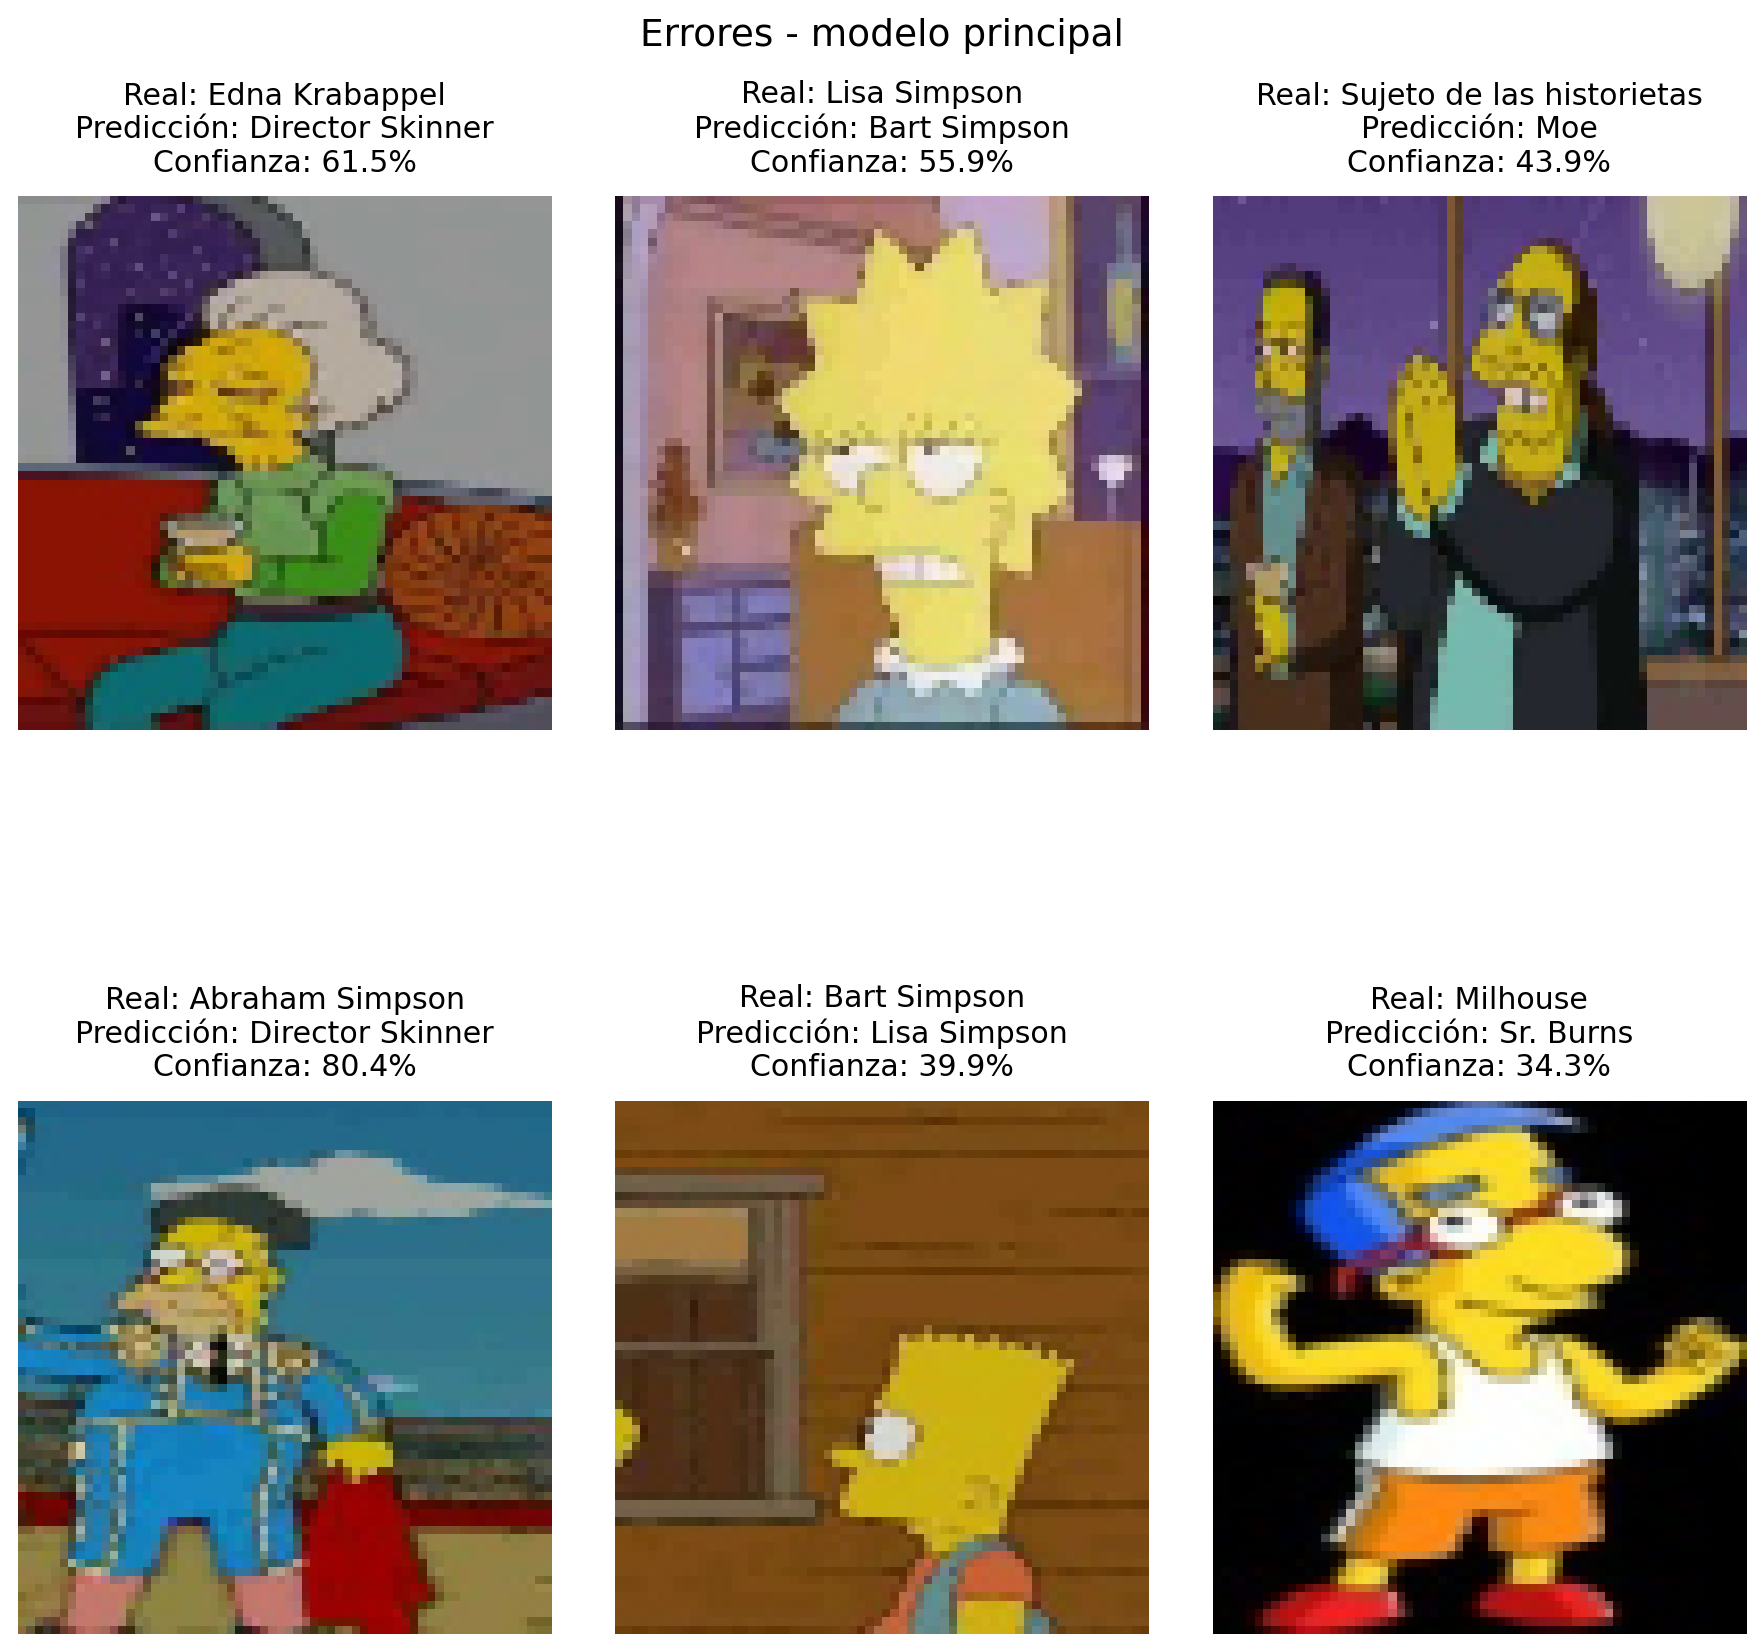
\includegraphics[width=0.95\linewidth]{errores.png}
\caption{Muestra del notebook: seis errores del RUN principal, con sus etiquetas de referencia, predicciones y confianza softmax.}
\label{fig:errores}
\end{figure}

\FloatBarrier
En la muestra de errores, Lisa aparece en primer plano y se predice Bart con confianza de 55,9\%. Abraham aparece con ropa y accesorios poco habituales y se predice Director Skinner con 80,4\%. Las imágenes también presentan cambios de encuadre, poses y escenas con varias figuras. Estas observaciones permiten identificar aspectos que revisar, pero el mosaico no basta para establecer las causas de los errores ni cuestionar las etiquetas.

Entre los 63 errores, 2 tienen confianza superior al 90\%, y ninguno de esos dos casos aparece en la muestra visual. La confianza media de los errores es 53,94\%. También hay aciertos con confianza más moderada, como Edna con 50,5\%.

Una salida softmax alta no garantiza que la predicción sea correcta. Tampoco se evaluó formalmente si esas probabilidades están calibradas, es decir, si se corresponden con la frecuencia real de aciertos. La confianza complementa la revisión del error y no reemplaza las métricas de desempeño.
\FloatBarrier

\section{Discusión y limitaciones}
D fue elegida con la regla definida. E quedó a 0,5352 puntos porcentuales en accuracy media y superó a D solo con semilla 123, mientras F empeoró las tres repeticiones. El efecto de cambiar la tasa depende de la configuración y de la semilla, por lo que estas diferencias se deben interpretar dentro del experimento realizado.

Una sola partición y tres semillas limitan la evidencia disponible. La validación se utiliza tanto para early stopping como para elegir la configuración. Por ello, sus métricas no permiten estimar de forma independiente el rendimiento en otras particiones. Las configuraciones se compararon por etapas, por lo que no se probaron todas las combinaciones posibles ni otros optimizadores. Las herramientas se justifican por su función, sin atribuirles mejoras que no se hayan evaluado.

El desbalance, las 18 clases seleccionadas y la reducción a $64\times64$ limitan el alcance del trabajo. El conjunto de prueba está casi equilibrado y obtiene resultados más favorables que validación, pero no se estudió por separado el efecto de su distribución ni el de la dificultad de las imágenes señalada en las sugerencias. Además, se mantiene el sobreajuste.

Probar imágenes externas y repetir D/E con otras semillas y particiones permitiría estudiar qué tan bien se generalizan los resultados. Estas pruebas quedan como trabajo futuro y no forman parte de los resultados obtenidos.

\section{Conclusiones}
Se adaptaron y documentaron dos arquitecturas del laboratorio para 18 clases y entradas de $64\times64$. Las seis configuraciones y tres semillas produjeron 18 RUN completos. En cada uno se recuperó el checkpoint de menor pérdida.

B mejoró A en 8,7216 puntos porcentuales de accuracy media de validación, con menos parámetros. Dropout mejoró esa base y D, con probabilidad 0,3 y Adam 0,001, obtuvo la mayor media, de 77,3186\%. Superó C en 1,7987 puntos porcentuales. Las tasas adicionales no mejoraron la media de D dentro del protocolo probado. E fue la alternativa más cercana, a 0,5352 puntos porcentuales.

El modelo principal \nombre{D_s42} alcanzó 92,9213\% de accuracy y 0,9298 de F1 macro en prueba. Las tres semillas promediaron 91,2360\%, con desviación de 2,0256 puntos porcentuales. Estos resultados respaldan D entre las alternativas evaluadas, considerando la variación entre entrenamientos, la representatividad del conjunto de prueba y la brecha de 18,3330 puntos porcentuales entre entrenamiento y validación.

\clearpage
\appendix
\section{Registro de los 18 RUN}
La época elegida corresponde al mínimo de pérdida de validación. Todas las detenciones fueron por early stopping. El tiempo corresponde a la llamada a \nombre{fit} y deja fuera el resto del proceso. Las métricas de esta tabla se obtienen con los pesos recuperados.

\small
\begin{longtable}{lrrrrrr}
\caption{Resultados individuales de los 18 RUN.}\label{tab:runs}\\
\toprule
RUN & Épocas & Elegida & Val. loss & Val. acc. (\%) & F1 macro & Tiempo (s) \\
\midrule
\endfirsthead
\toprule
RUN & Épocas & Elegida & Val. loss & Val. acc. (\%) & F1 macro & Tiempo (s) \\
\midrule
\endhead
\midrule
\multicolumn{7}{r}{Continúa en la página siguiente.}\\
\endfoot
\bottomrule
\endlastfoot
\csvreader[late after line=\\]{../resultados/entrenamientos.csv}{id=\identificador,epocas=\epocas,mejor_epoca=\mejorepoca,val_loss=\perdida,val_accuracy=\accuracy,val_f1_macro=\fmacro,segundos=\segundos}{%
\texttt{\expandafter\detokenize\expandafter{\identificador}} & \epocas & \mejorepoca & \numero{\perdida} & \escalado{100}{\accuracy} & \numero{\fmacro} & \numero[2]{\segundos}}
\end{longtable}
\normalsize

\end{document}
